%%
%% This is file `./samples/shortsample.tex',
%% generated with the docstrip utility.
%%
%% The original source files were:
%%
%% apa6.dtx  (with options: `shortsample')
%% ----------------------------------------------------------------------
%% 
%% apa6 - A LaTeX class for formatting documents in compliance with the
%% American Psychological Association's Publication Manual, 6th edition
%% 
%% Copyright (C) 2011-2017 by Brian D. Beitzel <brian at beitzel.com>
%% 
%% This work may be distributed and/or modified under the
%% conditions of the LaTeX Project Public License (LPPL), either
%% version 1.3c of this license or (at your option) any later
%% version.  The latest version of this license is in the file:
%% 
%% http://www.latex-project.org/lppl.txt
%% 
%% Users may freely modify these files without permission, as long as the
%% copyright line and this statement are maintained intact.
%% 
%% This work is not endorsed by, affiliated with, or probably even known
%% by, the American Psychological Association.
%% 
%% ----------------------------------------------------------------------
%% 
\documentclass[jou]{apa6}

\usepackage[american]{babel}

\usepackage{csquotes}
\usepackage[style=apa,sortcites=true,sorting=nyt,backend=biber]{biblatex}
\DeclareLanguageMapping{american}{american-apa}
\addbibresource{bibliography.bib}


%%%%%%%%%%%%%%%%%%%%%%%%%%%%%%%%%%%%%%%%
%% Discrete Structures
%% The start of RBS stuff
%%%%%%%%%%%%%%%%%%%%%%%%%%%%%%%%%%%%%%%%

% Working internal and external links in PDF
\usepackage{hyperref}
% Extra math symbols in LaTeX
\usepackage{amsmath}
\usepackage{gensymb}
\usepackage{amssymb}
% Enumerations with (a), (b), etc.
\usepackage{enumerate}

\let\OLDitemize\itemize
\renewcommand\itemize{\OLDitemize\addtolength{\itemsep}{-6pt}}

\usepackage{etoolbox}
\makeatletter
\preto{\@verbatim}{\topsep=3pt \partopsep=3pt }
\makeatother

% These sizes redefine APA for A4 paper size
\oddsidemargin 0.0in
\evensidemargin 0.0in
\textwidth 6.27in
\headheight 1.0in
\topmargin -24pt
\headheight 12pt
\headsep 12pt
\textheight 9.19in

\setlength\parindent{0pt}

\title{Quiz for Week02}
\author{Discrete Structures, Fall 2020}
\affiliation{RBS}

\leftheader{Discrete Structures Lab01: Hints}

\abstract{%
}

%\keywords{}

\begin{document}
%\maketitle

\twocolumn
{\Large Lab03: KMP and BM Matching}

\thispagestyle{empty}

In this lab you will create two Scala classes {\tt lv.rbs.ds.lab03.KMPmatcher}
and {\tt lv.rbs.ds.lab03.BMmatcher} that implement Knuth-Morris-Pratt and 
Boyer-Moore algorithms respectively and output the JSON data structures
that can be used to demonstrate step-by-step behavior of this algorithm. 

Both algorithms are widely known and practically important, and there are many implementations available
in the Internet (including in Scala), but in this lab assignment we add 
one more twist \textendash{} our goal is to show the ``debug-like'' behavior of 
both string matchers. See these animations:\\
\url{http://whocouldthat.be/visualizing-string-matching/}\\
\url{https://people.ok.ubc.ca/ylucet/DS/KnuthMorrisPratt.html}\\
\url{https://people.ok.ubc.ca/ylucet/DS/BoyerMoore.html}

To make your task more manageable, our goal is NOT a fully-functional Web application
that would perform these tasks, but only a simple backend to support such Web applications. 
Below we define the two classes (with their respective public APIs that you should implement.

\section{KMP Matcher}

\begin{verbatim}
class KMPmatcher:
  new KMPmatcher(pattern: String)
  def getPrefixFun(): List[Int]
  def findAllIn(text: CharSequence): 
        Iterator[Int]
  def toJson(text: CharSequence): String
\end{verbatim}

\begin{itemize}
\item {\tt KMPmatcher(pattern:String)} is a constructor to 
initialize a class instance. Since there are some initialization costs
related to the preprocessing of the searchable {\tt pattern}, 
it might be beneficial to reuse the same matcher with the same 
pattern to search multiple texts. We therefore avoid passing 
the target {\tt text} right away.
\item {\tt getPrefixFun()} returns the prefix function $\pi(j)$ (for $j=0,\ldots,m$), 
where $m$ is the length of the searchable pattern. 
Prefix function is the key data structure used by the KMP algorithm. 
It is returned as a list of integers. So the length of this
list is $m+1$.
\item {\tt findAllIn(text: CharSequence)} returns an iterator of 
offsets in the {\tt text} where the searchable {\tt pattern} starts. 
Please note that in the LAB03 you have to return {\bf all} offsets; 
it is not sufficient to find just the first instance and then give up.
\item {\tt toJson(text: CharSequence)} in this case we return a 
JSON data structure as in the provided JSON samples.
\end{itemize}


\section{Boyer-Moore Matcher}

\begin{verbatim}
class BMmatcher:
  new BMmatcher(pattern: String)
  def getGoodSuffixFun(): List[Int]
  def getBadCharFun(): List[(Char,Int)]
  def findAllIn(text: CharSequence): 
        Iterator[Int]
  def toJson(text: CharSequence): String
\end{verbatim}

This is similar to the previous class. The only difference is that 
JSON would now be different (since the Boyer-Moore matching has 
every step scanning backwards: $\mathtt{start} \geq \mathtt{end}$.
Also the two data structures (Good Suffix function and Bad Character function) 
are peculiar to this type of matching. 

\section{JSON sample for KMP}

\begin{verbatim}
{
  "algorithm": "KMP",
  "pattern": "ABCDABD",
  "text": "ABC ABCDAB ABCDABCDABDE",
  "prefixFun": [[0,-1],[1,0],[2,0],[3,0],
    [4,0],[5,1],[6,2],[7,0]],
  "steps": [
    { "offset": 0, "start": 0, "end": 3 },
    { "offset": 3, "start": 0, "end": 0 },
    { "offset": 4, "start": 0, "end": 6 },
    { "offset": 8, "start": 2, "end": 2 },
    { "offset": 10, "start": 0, "end": 0 },
    { "offset": 11, "start": 0, "end": 6 },
    { "offset": 15, "start": 2, "end": 6, 
	    "match": "true" },   
    { "offset": 22, "start": 0, "end": 0 }
  ]
  "comparisons": 27
}
\end{verbatim}

\section{JSON sample for BM}

\begin{verbatim}
{
  "algorithm": "BM",
  "pattern": "ABCDABD",
  "text": "ABC ABCDAB ABCDABCDABDE",
  "goodSuffixFun": [[0,-7],[1,-6],[2,-5],
      [3,-4],[4,-3],[5,2],[6,5]],
  "badCharFun": [["A",4],["B",5],["C",2],["D",6]],	
  "steps": [ 
    { "offset": 0, "start": 6, "end": 6 },
    { "offset": 4, "start": 6, "end": 6 },
    { "offset": 11, "start": 6, "end": 6 },
    { "offset": 15, "start": 6, "end": 0, 
        "match": "true" }    
  ],
  "comparisons": 10
}
\end{verbatim}



\end{document}

\newpage

\section{Project Setup Steps}


\subsection{Create Empty Project (Instructor only)}

The instructions are given for Windows 10
(assume that Instructor likes to use Eclipse Scala IDE \textendash{} 
see \url{http://scala-ide.org/}). 
Instructions for Linux and IntelliJ IDEA would be different.

\begin{enumerate}[(1)]
\item Install sbt ({\em Simple Build Tool}). See \url{https://bit.ly/2UzE8hj} for details.
\item Run this command in any directory that does
not already contain subdirectory {\tt ds-lab03}. 
Create an empty project from a template, name it {\tt ds-lab03}, 
change your directory to that project and run {\tt sbt} commandline
from the project's root directory:
\begin{verbatim}
sbt new scala/hello-world.g8
Name: ds-lab03
cd ds-lab03
sbt
\end{verbatim}
\item Create Eclipse project files and run the empty (hello world) project
created by the template; then exit the SBT session:
\begin{verbatim}
eclipse
run
exit
\end{verbatim}
\item Initialize a project in Eclipse Scala IDE: 
\begin{center}
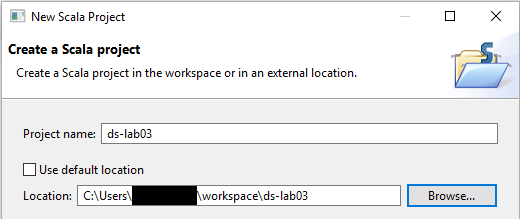
\includegraphics[width=2.5in]{lab03/eclipse-new-project.png}
\end{center}
\end{enumerate}


\subsection{Add scalatest testcases}





